\chapter{Introduction}
\thispagestyle{empty}
\label{chap:intro}
    
    \pagestyle{fancy}
    \renewcommand{\chaptermark}[1]{ \markboth{#1}{} }
    \renewcommand{\sectionmark}[1]{ \markright{#1}{} }
    \fancyhead{}
    \fancyhead[R]{\leftmark}
    \fancyhead[R]{\rightmark}
    \fancyfoot{}
    \renewcommand{\footrulewidth}{0.4pt}
    \fancyfoot[R]{\thepage}

In recent years, the competition between coherent and dissipative dynamics in many-body quantum systems has been studied, which has led to the emergence of novel types of dynamical phase transitions known as measurement-induced phase transitions (MIPTs) \cite{li2018,li2019,chen2020,skinner2019,bao2020,jian2020,zabalo2020,zhang2020,gullans2020,bentsen2021a}.  In chapter~~\ref{chap:MIPT_bosons}-\ref{chap:short_time_dynamics}, we study this competition between coherent and dissipative dynamics in continuous time models and analyze some scenarios in which MIPTs arise. We begin by providing a brief overview and introducing this novel transition type.

\section{Overview}

The field of quantum many-body physics explores emergent properties of ensembles of many quantum particles, such as atoms, electrons, or photons, interacting with each other according to the laws of quantum mechanics. These systems can give rise to new exciting physics, such as the behavior of ultra-cold atomic gases in optical lattices \cite{bloch2012} or the emergence of novel phases of matter in condensed matter systems \cite{bernevig2013}.

The interplay of quantum mechanics of how particles interact in quantum many-body systems leads to novel and often unexpected phenomena, such as quantum phase-transitions, high-temperature superconductivity \cite{leggett2006}, thermalization \cite{srednicki1994} and novel states of matter such as superfluidity \cite{schmitt2015} or Bose-Einstein condensation \cite{georgescu2020}, which have both fundamental significance and potential technological applications.

Furthermore, quantum many-body physics plays a vital role in investigating fundamental problems in fields such as quantum information theory. For example, exploring the entanglement structure of quantum many-body states gives valuable insight into the potential use in quantum information processing tasks \cite{luecke2014, schmied2016, luo2017}. Quantum entanglement is an interesting property of quantum many-body states, as it characterizes the non-classical correlations in the system. When two or more quantum systems are entangled, their properties, such as spin or polarization, become correlated so that the state of one system instantaneously affects the state of the others, regardless of the distance between them. Such non-local correlations challenge classical intuition and form the basis of various quantum technologies, including quantum cryptography, quantum teleportation, and quantum computing. A quantum many-body system is said to be entangled when the quantum states of individual particles that make up the system cannot be described independently of the state as a whole \cite{nielsen2000}. In other words, if the wave function of the system cannot be written as the product of the wave function of two subsystems that make up the whole system, then these subsystems are entangled. 

\begin{figure}[ht]
    \centering
    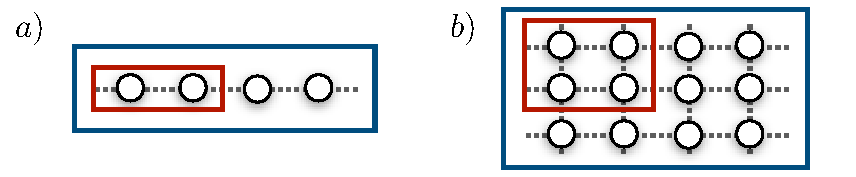
\includegraphics[width=\textwidth]{Chapters/Plots/Chapter1/Chapter0_Fig2.pdf}
    \caption{Schematic representation of a quantum many-body system consisting of particles on a lattice in a) 1D and b) 2D. The blue boundary denotes the total quantum system, and the red boundary denotes a subsystem of the total quantum system.} 
    \label{fig:Chapter0_Fig2}
\end{figure}

Mathematically, we formulate this as $\ket{\psi_{AB}} \neq \ket{\psi_A} \ket{\psi_B}$, where $\ket{\psi_{AB}}$ denotes the wave function of the whole system, and $\ket{\psi_A}, \ket{\psi_B}$ denote the wave functions of the subsystems A and B, respectively. In contrast, if a quantum system is not entangled, it is possible to express it as the product of subsystems, $\ket{\psi}_{AB} = \ket{\psi}_A \ket{\psi}_B$, and we can fully describe either subsystem independently of the system as a whole. For this reason, such states are also known as separable states. Quantum entanglement has a range of useful applications, such as in quantum cryptography \cite{pirandola2020}, where entangled states can be used for quantum key distribution protocols (see, e.g., \cite{ekert1991}) that ensure that nobody intercepted the communication. Entanglement provides a sensitive probe, such as for quantum thermalization \cite{deutsch1991,rigol2008,dalessio2016}, information scrambling \cite{srednicki1994,trail2008,bentsen2019}, or the characterization of quantum phases \cite{calabrese2004}.

In quantum information processing, entanglement is connected to quantum resource theories, defined by some operations classes. Choosing, for instance, local operations and classical communication as the set of operations that can be used, only separable (non-entangled) states can be created under this class \cite{horodecki2013}. Since entangled states cannot be created under this class of operations, they become a resource as they cannot be created for 'free'. Given entangled states, however, performing tasks that would otherwise not be possible via the allowed operations becomes possible~\cite{nielsen,horodecki2009,horodecki2013}. Entanglement measures provide useful ways to quantify how much entanglement (or, in other words, quantum correlations) there is (are) in a system \cite{plenio2006}, and one important measure is the von Neumann entropy ($S_{VN}$), which we will use throughout this thesis. The von Neumann entropy is an entanglement measure that quantifies the amount of entanglement present in a pure system. Let us consider again a quantum state $\hat{\rho}_{AB} = \ket{\psi_{AB}}\bra{\psi_{AB}}$, where A and B denote two subsystems that make up the whole system. To quantify the amount of entanglement present between the two subsystems, $A$ and $B$, we can use the von Neumann entropy of the reduced system $S_{VN}(\hat{\rho}_A) = S_{VN}(\Tr_B(\hat{\rho}_{AB}))$, where $\Tr_B$ denotes the partial trace over the subsystem $B$. 

Computational simulation of quantum many-body systems dynamics is challenging as the Hilbert space in which quantum states live grows exponentially with the number of particles in the system. In a system that consists of $n$ 2-level systems, $2^n$ complex coefficients are needed to describe the state fully. Consequently, for simulations, $2^n$ complex numbers must be stored in a computer, which quickly becomes impossible for many particles. In quantum computing \cite{forcer2002, nandhini2022}; however, a superposition of $2^n$ states can be represented using $n$ 2-level systems, which can lead to exponential speed-ups for certain problems and is also known as quantum parallelism. Moreover, entanglement plays a vital role in quantum computing, as it has been shown that to achieve exponential speed-up over classical computation, multipartite entanglement (i.e., entanglement between more than just two subsystems) is needed in the system \cite{jozsa2003}. One of the most well-known algorithms benefitting from this exponential speed-up is Shor's algorithm for factoring numbers into their prime factors\cite{shor1997}.

\begin{figure}[ht]
    \centering
    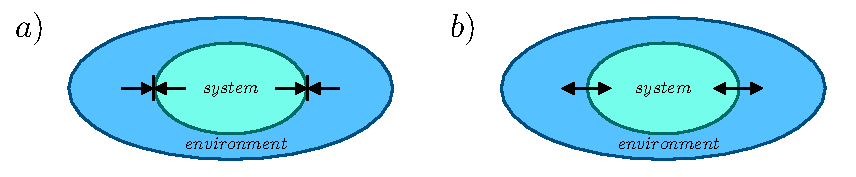
\includegraphics[width=\textwidth]{Chapters/Plots/Chapter1/Chapter0_Fig4.pdf}
    \caption{Schematic representations of a) a closed and b) an open quantum system. The closed quantum system does not interact with the environment nor exchange matter or energy, as indicated by the arrows blocked by the solid black lines. In contrast, an open quantum system does interact with its environment. It is a more realistic representation, as it is essentially impossible to guarantee that no energy or particles leave the system of interest.}
    \label{fig:Chapter0_Fig4}
\end{figure}

The closed system behavior of a many-body quantum system is prescribed by the Schr\"{o}dinger equation, leading to the description of the unitary time evolution of the density operator. Moreover, in isolated systems that thermalize, the entanglement entropy of a subsystem is extensive \cite{nandkishore2015}, corresponding to linear growth of entanglement entropy with subsystem size in $1D$, also known as \textit{volume-law} scaling of the entanglement entropy. 

In reality, however, no quantum system is ever truly isolated, leading to dissipative processes that prevent the system from evolving unitarily. Such dissipative processes can occur either as a result of measurements being voluntarily performed by an observer or simply due to the coupling to the environment, resulting in loss of information. More specifically, local measurements (such as projective measurements) tend to decrease the amount of entanglement present in the system by projecting the wave function on a given site to be in a definite state, effectively disentangling it from the rest of the system. One question that arises is whether or not the volume-law scaling of the entropy in thermalizing systems survives when local measurements are performed, as they reduce the total amount of entanglement present in the system. 

\begin{figure}[ht]
    \centering
    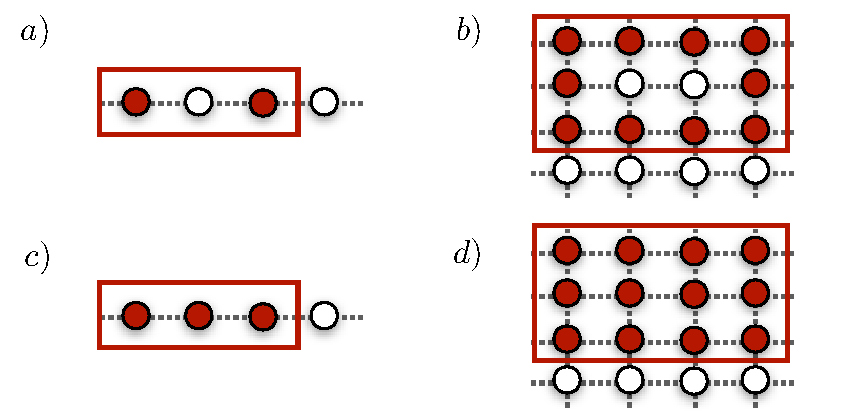
\includegraphics[width=\textwidth]{Chapters/Plots/Chapter1/Chapter0_Fig3.pdf}
    \caption{Schematic representation of the area of the boundary in a) $1D$ and b) $2D$, and the volume of the boundary in c) $1D$ and d) $2D$. In $1D$, the area will remain constant, no matter how much the subsystem grows, as only one (or two if one considers periodic boundary conditions) cut(s) are needed to divide the system into two subsystems. Therefore, if the entropy is constant with subsystem size, we call this area-law, as we will see in later chapters. On the other hand, the volume consists of all the particles contained within the subsystem, which grows linearly as the subsystem grows. We, therefore, speak of volume-law entanglement when the entropy grows linearly with the subsystem size. Similarly, in $2D$, the area grows linearly with subsystem size while the volume grows quadratically, and analogous to the $1D$ case, one speaks of area and volume-law scaling of the entropy when the entropy of the subsystem scales either linearly or quadratically with the boundary.}
    \label{fig:Chapter0_Fig3}
\end{figure}

As we have discussed, having access to quantum states that withstand disentangling dynamics is particularly useful for quantum computers and simulators, where entangled states serve as an important resource. Therefore, it is important to understand the effect of measurements on unitary dynamics, as it allows us to characterize the entanglement properties of states in novel dynamical quantum phases that may be employed in quantum computers.

The competition between coherent and local dissipative dynamics has led to the notion of measurement-induced phase transitions (MIPTs), which were first discovered in random circuits. The competition arises because coherent dynamics can build up the total amount of entanglement in the system, while local dissipative dynamics tend to decrease it. We will now provide a brief overview of MIPTs in the context of random circuits before we discuss them in continuous time models.

\subsection{MIPTs in Random Circuits}

 MIPTs have been explored in recent years in random circuit models \cite{li2018,li2019,skinner2019,bao2020,jian2020,zabalo2020,zhang2020,lang2020, moghaddam2023,martin-vazquez2023} where it has been shown that continuous phase transitions arise as a result of the competition between entangling unitary dynamics and disentangling local measurements. These transitions are characterized by the qualitative change in the wave function undergoing a measurement trajectory, making it crucial to track measurement outcomes.

\begin{figure}[ht]
    \centering
    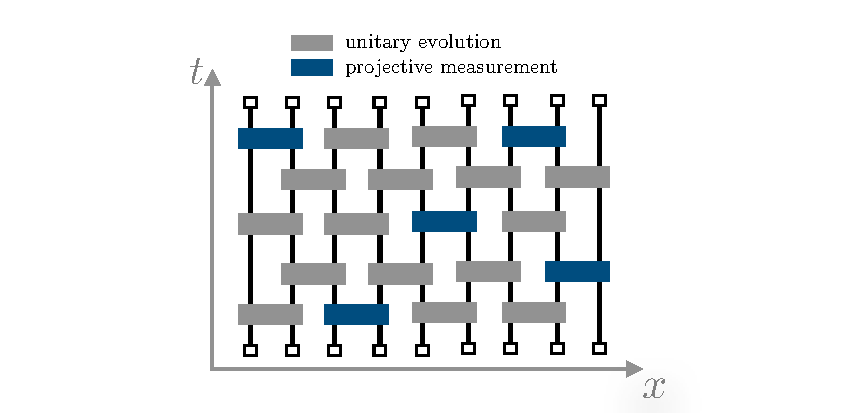
\includegraphics[width=\textwidth]{Chapters/Plots/Chapter1/Chapter0_Fig5.pdf}
    \caption{Schematic representations of hybrid circuit model. The unitary gates (gray) are applied pairwise on neighboring qubits. The projective measurements (blue) are applied randomly in time (t) and space (x) before applying the unitary gates.}
    \label{fig:Chapter0_Fig5}
\end{figure}

Refs.~\cite{li2018,li2019,skinner2019} present a phase transition in a hybrid circuit model (Fig.~\ref{fig:Chapter0_Fig5}), where an initial non-entangled product state is time-evolved by applying random unitary gates drawn from various distributions. The unitary evolution is interrupted by performing projective measurements randomly in time and space with a probability $p$ per unitary gate. No projective measurements occur for $p \to 0$, while for $p \to 1$, projective measurements are applied before each unitary gate. The entanglement grows over time with this model, and the steady-state exhibits volume-law scaling of the entanglement entropy for small measurement probabilities, indicated by linear growth of the entropy with the subsystem size. Then, at a critical measurement probability, it undergoes a phase transition into a ``quantum Zeno'' regime \cite{itano1990}. In this regime, measurements occur frequently, suppressing the entanglement growth, resulting in the area-law scaling of the entropy, where the entropy is constant and independent of the subsystem size.

As mentioned before, these transitions are characterized by qualitative changes in the measurement trajectories, and it is important to note that at the level of the density operator, this transition is masked. As the measurement outcomes are random, after a long time evolution, each local measurement outcome is obtained roughly equally. This has the consequence that upon averaging over all measurement outcomes, any state in the Hilbert space is equally likely corresponding to an infinite temperature state. For any nonzero measurement probability, given enough time, the infinite temperature state is reached, and therefore, the transition is not accessible. 

Other types of transitions have also been explored in random circuits, such as purification transitions \cite{gullans2020,bentsen2021a} where an initially mixed state is time evolved while subjected to continuous measurement. As the measurements destroy quantum correlations between subsystems, the entropy also decreases. Above a critical measurement strength, the average entropy decays to zero independent of the system size, implying that as a result of the measurements, we know what the state of the system is. Below the critical measurement strength, the entanglement is not entirely destroyed, and the time to purify the system grows exponentially with the system size.  

Not only are these transitions of fundamental interest, but they can also be related to the generation of error correction codes in quantum channels \cite{choi2020,gullans2021,fan2021,li2021}, where they arise during the unitary time evolution and protect the volume-law phase against disentangling projective measurements. Furthermore, there has been progress in probing these entanglement transitions \cite{gullans2020a,noel2022}. In Ref.~\cite{gullans2020a}, the authors propose the entropy of a reference qubit entangled with a system of interest as an order parameter for a MIPT. Below the critical measurement strength, the entropy of the reference qubit can stay nonzero while it decays to zero above the critical measurement strength. In Ref.~\cite{noel2022}, the authors probe the transition using the probe proposed in \cite{gullans2020a} on a trapped-ion quantum computer and find experimental evidence of the two phases by measuring the entropy of the reference qubit.

\subsection{MIPTs in Continuous Time Models}

\begin{figure}[ht]
    \centering
    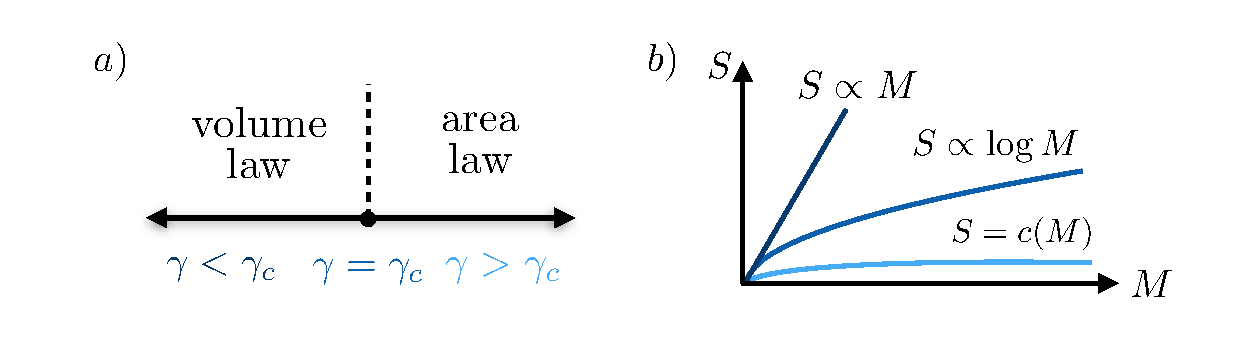
\includegraphics[width=\textwidth]{Chapters/Plots/Chapter1/Chapter0_Fig1.pdf}
    \caption{a) Schematic representation of a phase diagram in a non-integrable model that exhibits a measurement-induced phase transition at a critical measurement strength $\gamma_c$ from volume law scaling of the entropy to area-law scaling. b) Schematic representation of the characteristic behavior of the entropy; close to criticality, the entropy scales logarithmically with the subsystem size $M$, the volume-law phase is characterized by linear growth of the entropy, and in the area-law phase, the entropy grows minimally and remains constant.}
    \label{fig:Chapter0_Fig1}
\end{figure}

As we have just discussed, random circuits have been explored in depth in recent years \cite{fisher2022}, and a natural question is whether the same entanglement transition can be seen in continuous time models. This type of transition has also been investigated in spin chains and bosonic systems \cite{fuji2020,tang2020,biella2021,doggen2022, botzung2021, muller2022}. Refs.~\cite{fuji2020,tang2020,doggen2022} investigate a bosonic system, where they break the integrability of the model to witness a stable volume-law scaling phase. They find an entanglement transition where a qualitative change from volume-law scaling to area-law scaling of the entropy occurs. The characteristic behavior of this transition is schematically represented in Fig.~\ref{fig:Chapter0_Fig1}. Integrable models tend to possess many symmetries \cite{retore2022}, which means they are exactly solvable. Non-integrable models, on the other hand, are not exactly solvable, and it has been shown that they exhibit volume-law scaling of the entanglement entropy \cite{nakagawa2018}. Interestingly, as we will see, MIPTs can arise in both integrable and non-integrable models. 

A chain of non-interacting free fermions has been shown to have no volume-law phase for arbitrarily small measurement strengths \cite{cao2019} and an area-law phase that is present for any nonzero measurement rates. It was later shown \cite{alberton2021} that the model exhibits a phase transition where the entanglement entropy scales logarithmically with the subsystem size for small but nonzero measurement rates. At a critical rate of the measurements, the system undergoes a phase transition beyond which the entropy exhibits area-law scaling. In later chapters, we will also analyze these transitions and discuss the difficulties of accurately identifying them. Some schemes have been proposed to observe these transitions, using pre-selection \cite{buchhold2022}, where the stationary state of the model can be altered by steering the system towards a specific state that does not destroy the underlying properties that result in the transition.

In Ref.~\cite{doggen2022}, a transition was predicted in the Ising model, where the transverse magnetization is monitored. Similar to other systems, a transition in the quantitative behavior of the wave function occurs; however, instead of using the entanglement entropy, they consider the overlap between the trajectory steady-state and the localized quantum Zeno product state, which characterizes at which point the dissipative dynamics take over.

\subsection{Challenges}

As previously mentioned, the MIPTs are masked at the density operator level for random circuits. In continuous models, where dissipation in the form of dephasing occurs, the steady-state obtained through averaging over all possible measurement outcomes is the trivial infinite temperature state, independent of measurement strength. Similarly, by considering the master equation, which describes such a system, it also always reaches the infinite temperature state, so we cannot directly use the master equation to find the signatures of MIPTs in steady-states of continuous time models. Instead, we need to consider non-linear quantities, such as the entanglement entropy at the quantum trajectory level, to access these transitions. These quantities need to be evaluated at the trajectory level before computing the average over all trajectories as linear quantities, which would again correspond to the expectation value in the infinite temperature state. Another challenge to overcome is to extract these non-linear quantities from individual trajectories, as generally, multiple measurements on a single trajectory are required to access these quantities. Suppose measurements are made deterministically in time and repeatable for specific measurement outcomes in these systems. In that case, it is theoretically possible to extract quantities like the entanglement entropy of subsystems by repeating trajectories and performing measurements with the interference of copies \cite{islam2015, daley2012} or random unitaries \cite{elben2018, brydges2019}. 

However, the measurement results are typically not reproducible - and more commonly, they are not even known when the dissipation comes from natural coupling to the environment or random noise. In this case, performing more than one measurement on a single trajectory is impossible, and techniques for extracting the entanglement entropy cannot be used. Here, we consider what can be realized in such realistic and also small, finite-sized systems corresponding, e.g., to current 1D experiments in quantum gas microscopes \cite{bakr2009, sherson2010, gross2021}. The random entangling gates are replaced by unitary dynamics of interacting dipolar bosons on a 1D lattice \cite{patscheider2020}. In contrast, the random measurements are replaced by local dephasing, which can be readily realized for ultracold gases through noise or light scattering~\cite{luschen2017,pichler2010,sarkar2014,poletti2013}. By looking at the trajectories corresponding physically to dephasing events at particular positions and locations, we can find a similar change in behavior moving between area- and volume-law entanglement growth as we change the dephasing rate. Investigating the steady-state properties of quantum trajectories will be the main focus of chapters \ref{chap:MIPT_bosons} and \ref{chap:MIPT_continuous_measurement}.

These difficulties are somewhat reduced when we relax the focus on steady-state dynamics and also consider short- or intermediate-time dynamics. In this case, at long times, the steady-state remains the infinite temperature state, and the master equation cannot be used to detect signatures of the MIPTs. Interestingly, however, by investigating how the system in question reaches the infinite temperature state, signatures of the transitions are present in both non-linear and linear quantities in the density operator. Obviously, for non-linear quantities, the order in which we compute the average and quantity still matters. However, this is not the case for linear quantities (such as the local densities), and here, in principle, the master equation approach can also be employed to investigate the system and gain information on the transition signatures. However, it is essential to note that the transition itself cannot be detected this way, as this is only possible in the steady-state where the master equation approach does not work. The signatures that are present at early and intermediate times are the focus of chapter \ref{chap:short_time_dynamics}. Although it is, in principle, possible to use the master equation approach in some cases that we just discussed, we continue to use the trajectory approach, as we are not only interested in the evolution of the average values but also in the statistics when many trajectories are simulated as we gain additional information from the statistics and how the quantities are distributed.

\section{Thesis Outline}

In chapter~\ref{chap:intro}, we have introduced the main background ideas that have inspired the work presented in this thesis. We introduced measurement-induced phase transitions in the context of random circuits where they were first studied and in continuous time models. \\

In chapter~\ref{chap:phase_sec}, we will discuss classical and quantum phase transitions to provide a brief overview of this topic. We will consider a simple example to introduce the main concepts that we need to study the phase transitions presented in the following chapters. \\

Chapter~\ref{chap:tech_sec} focuses on the main tools and methods used to simulate open quantum systems numerically. We outline the derivation of the Lindblad master equation, which describes the time evolution of an open quantum system subject to dissipative processes. We then introduce the Monte Carlo wave function method to simulate the master equation more efficiently. Finally, we discuss homodyne detection and quantum state diffusion, which provide another unraveling of the master equation, also allowing us to simulate the master equation numerically.  \\

In chapter~\ref{chap:MIPT_bosons}, we study a chain of interacting hardcore bosons subject to dephasing. We present a measurement-induced phase transition that arises from the competition between coherent and dissipative processes manifesting in the entanglement entropy. We use the main ideas introduced in chapter~\ref{chap:intro}-\ref{chap:phase_sec} to characterize the phase transition and highlight the limitations we encounter in the model. We also provide a detailed discussion on the scaling collapses for the system sizes we can simulate and turn to free fermions to allow for the simulation of larger systems. Finally, we explicitly break the $U(1)$ symmetry conserved in the model and investigate whether we still see this phase transition. \\

In chapter~\ref{chap:MIPT_continuous_measurement}, we attempt to find a way to witness the quantum phase transition experimentally, which is no easy task as the quantities witnessing the transition need to be non-linear in the density operator. We show for a class of correlation functions how this rules out the possibility of measuring them experimentally. \\

In chapter~\ref{chap:short_time_dynamics}, we relax the constraints of focusing exclusively on steady-state properties by considering non-linear as well as linear quantities at early times. We show that signatures of the competition between coherent and dissipative dynamics can be resolved even at early times. This allows us to propose an experimental protocol that can probe the competition between coherent and dissipative dynamics in the model. \\

In chapter\ref{chap:conclusion}, we conclude the thesis and summarize what we have learned by undertaking the projects discussed in chapter~\ref{chap:MIPT_bosons}-\ref{chap:short_time_dynamics}. 
